\documentclass[a4paper, 11pt]{article}
\usepackage[a4paper, left=1.2in, right=1.2in, top=1in]{geometry} %less whitespace
\usepackage{graphicx} 				%Include figures
\graphicspath{ {figures/} } 		%Path where images are stored
\usepackage[scaled]{helvet} 		%Helvetica font
\renewcommand\familydefault{\sfdefault} 
\usepackage[utf8]{inputenc}
\usepackage{url}                    %link and format URLs
\usepackage[multiple]{footmisc} 	%comma separated footnote references
\usepackage[numbers]{natbib} 		%Alt. bibliography (print author / year stile in text)
\usepackage{enumitem}				%make lists / dictionarys
\usepackage{algorithm} 				%for pseudocode
\usepackage{algpseudocode} 			%for pseudocode
\usepackage{subcaption}				%to include subfigures

\begin{titlepage}
\title{\textbf{Cochlear Implant Electrode Detection (CIED)}}
\author{Tim Ogi, Lucien Hinderling, Dona Lerena}
\end{titlepage}


\begin{document}
\maketitle
\section{Introduction}
Nowadays, profound hearing losses are most commonly treated with cochlear implants (CIs), which can restore the hearing by directly stimulating the auditory nerves with electrical impulses. A CI system consists of 1) an external audio processor, 2) the transmission coil, 3) the receiver/stimulator unit and 4) the electrode array, which is inserted into the cochlea. As the cochlea is organized tonotopically, the position of the inserted electrodes is of atmost importance to estimate how a particular frequency is perceived by the patient. Therefore, the aim of this project is to determine the angular depth of the 12 inserted electrodes, using pre-and postoperational computer tomography (CT) images from multiple patients.


\section{Methods}
\subsection{Ground truth creation}
\subsection{Electrode detection and labeling}
This chapter describes how the electrodes are detected and labeled from innermost to outermost. 
\subsubsection{Preprocessing}
The images are normalized using contrast stretching. First a lower and upper bound of the input image histogram specified, we chose the 2nd and 98th percentile. Values outside of this range are ignored in the calculation to be robust against outliers. The lower and upper bound are set as the new minimum and maximum brightness, a linear transformation is applied to stretch the intensity values over the whole dynamic range of our dataype. This function improves the contrast of low contrast images without distorting the relative intensities, while high contrast images remain mostly unchanged\footnote{\url{http://homepages.inf.ed.ac.uk/rbf/HIPR2/stretch.htm}}\footnote{\url{https://scikit-image.org/docs/0.9.x/auto_examples/plot_equalize.html}}. This step is necessary as treshold is applied on the response value of the following blob detection, which is dependent on the absolute image intensities.

\subsubsection{Blob detection}
To detect bright spots in the image which could represent electrodes, blob detecion laplacian of gaussian (LoG) blob detection is applied. It was selected over other implementations of the blob detection, as it provides the most accurate results\footnote{\url{https://scikit-image.org/docs/dev/auto_examples/features_detection/plot_blob.html}} and computation speed is not a criterion. The second derrivatives of gaussian kernels with different sigma values are convoluted with the input image. For each image location the response value and the sigma value with which the highest response was achieved are stored. The results are filtered a) to only contain gaussian responses of certain sigma values, representing the size of the electrodes, and b) to only contain responses of a certain intensity, which filters out the response to image noise or other blob-like structures with weaker intensities than the electrodes we are interested in. A implementation\footnote{\url{https://scikit-image.org/docs/dev/api/skimage.feature.html#skimage.feature.blob_log}}.
provided by the \emph{scikit-image} \cite{scikit-image} library was used.
See figure \ref{blobs_detected} as an example of an output. The treshold was intentionaly set low, so blobs can also be detected in images where the electrodes are differentiated weaker.

\begin{figure}[ht]
	\centering
  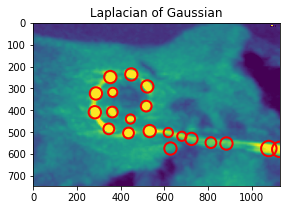
\includegraphics[width=.5\textwidth]{blobs_detected.png}
	\caption{Image after contrast stretching. Red circles indicate locations where blobs have been detected. Radii are aproximated using $r=\sqrt{2\sigma}$.}
	\label{blobs_detected}
\end{figure}

\subsubsection{Blob selection and labeling with MLE}
The next question is to filter the electrodes from all detected blobs and to find a path that connects them all, so they can be labeled from 1 to 12 accordingly.  
As the information of the pattern to be recognized is mostly structural, a graph approach comes naturally. Some key information available on the electrodes can be boiled down to these points:

\begin{description}[] %Info
\item[Electrode shape and intensity] The electrodes apper in a round shape and are brighter than the surrounding tissue. This information is already encoded in the model for blob detection.
\item[Electrode count] There are exaclty 12 electrodes to be detected in every image
\item[Equidistance] The all distances between two adjacent electrodes are the same, as they are fixed onto the wire inserted in the cochlea in a regular pattern. Except the first and last electrode, all electrodes have exaclty two neighbors. 
\item[Spiral shape] The wire inserted follows the form of the cochlea and has a spiral shape. The chochlea turns in a regular pattern and has no sharp angles. The electrode desity is highest in the cochlea where the turns get tighter.
\end{description}
Blobs are removed sequentially until only a certain amount of blobs $n$ remain. %TODO Tim
A graph representation is created using the \emph{networkX} library \cite{networkx} by assuming each detected blob to be a node. Two blobs are connected with an edge if the distance between them falls into an empirically determined range (see fig. \ref{network_raw}). %TODO Dona

\begin{figure}[ht]
	\centering
  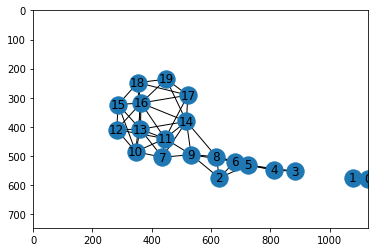
\includegraphics[width=.5\textwidth]{network_raw.png}
	\caption{The initial graph constructed from the blobs in figure \ref{blobs_detected}. The unconnected subgraph containing node 1 will be removed in the following step, see figure \ref{graphs}}
	\label{network_raw}
\end{figure}

Disconnected subgraphs containing less than 12 electrodes are removed.
A set of valid paths is generated by using the information of the electrode cound and spiral shape: Two neighbouring nodes are chosen as starting nodes (this is repeated for all $n$ nodes and all their neighbors). The two starting nodes are used as initialization values of $path_{1...i = len(path)} $ the following recursive function:

\begin{algorithm}[H]
	\caption{findpath($graph,path$)} 
	
	\begin{algorithmic}[1]
		\If{$len(path)$ = 12}
			 \State We have found 12 electrodes.
		\Return $path$
		\EndIf
		\State For the node added last to the $path$ check if they have neighbors.
		\For {$node = [all\ neighbours\ of\ path_i, \notin path]$}
				\State Check if we make a plausible turn by choosing this node as continuation of our path:
				\State $\alpha$ = angle between $\overrightarrow{path_i-1, path_i}$ and $\overrightarrow{path_i, node}$
				\If{$\alpha$ $<$ empirically determined treshold}
					\State A new possible way to continue this graph has been found, the turn is not to sharp.
					\State $path_{new}$ = Add $node$ to $path$
					\State Recursively call this function with the new path:
					\State \emph{findpath}($graph,path_{new}$)
				\EndIf
		\EndFor
		\If{$node = [\ ]$}
			\State There is no way to continue this path
			\Return
		\EndIf
		
	\end{algorithmic} 
\end{algorithm}

This leads to a set of paths $P$ where each path $p_i \in P$ is valid to the constraints of having exaclty 12 nodes and not making impossible turns. Now we filter the paths by assigning a cost function $c_a$ encoding our knowledge about the equidistance of the path: The cost is the variance of the length of all the edges connecting the 12 electrodes in the path $p_i$
$$ c_a(p_i)=var(edges\in p_i)$$
These values were then normalized with min-max normalization for each image. The path with the loest cost was accepted as the right solution, giving us not only the 12 right nodes, but also the order in which they are connected.
This already led to really good results in most of the images of the test set, except in two images where there was another path which had a lower edge length variance than the expected solution. These paths started further out, by wrongly assuming part of the wire leading to the outermost electrode as an electrode. To penalize these solutions, a second cost function $c_b$ was introduced, that measured the "compactness". It works by summing up all distances of each node to the mean location of all 12 nodes, assigning less cost to solutions that are nicely curled up, and more cost to solutions that are stretched out. 

$$ c_b(p_i)=dist (nodes \in p_i\ to\ center\ of\ mass)$$
The two cost functions are combined into $c_ {c}$. One can think of it as the euclidean distance of the two cost functions from the null point in figure \ref{feature_distribution}.

$$c_{c} = \sqrt{c_a^2+c_b^2}$$

The distribution of $c_a$ and $c_b$ for all valid paths detected in one image are illustrated in figure \ref{feature_distribution}.

\begin{figure}[ht]
	\centering
  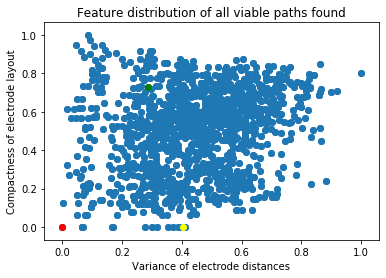
\includegraphics[width=.5\textwidth]{feature_distribution.png}
	\caption{Costs of all paths found in an image. Three paths are highlighted to better illustrate what the dots stand for, and are pictured in the subsequent figures. \textbf{Red:} Best path found (lowest cost for $c_c$), \textbf{Yellow, Green:} Randomly selected.}
	\label{feature_distribution}
\end{figure}


\begin{figure}[ht]
\begin{subfigure}[c]{0.32\textwidth}
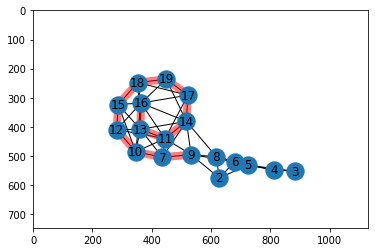
\includegraphics[width=1\textwidth]{best_path.png}
\subcaption{Best path found}
\end{subfigure}
\begin{subfigure}[c]{0.32\textwidth}
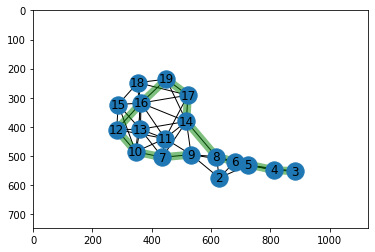
\includegraphics[width=1\textwidth]{random_path_1.png}
\subcaption{Randomly selected path}
\end{subfigure}
\begin{subfigure}[c]{0.32\textwidth}
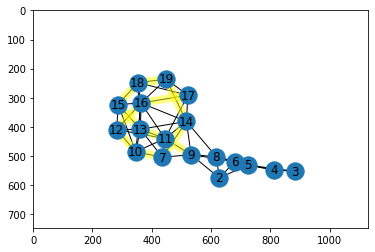
\includegraphics[width=1\textwidth]{random_path_2.png}
\subcaption{Randomly selected path}
\end{subfigure}
\caption{Paths taken from the feature distribution illustrated in figure \ref{feature_distribution}}
\label{graphs}
\end{figure}
This procedure meant each path was detected twice (forwards and backwards). To calculate the angles it is necessary to start counting at the right node. The starting node was decided by comparing the distance to the electrode center of mass for the first and last node in path.

\subsection{Spectral center}
The spectral center has been approximated as the center of the circle built by the three innermost electrodes.
$$\overrightarrow{M1}+s*\overrightarrow{n1}=\overrightarrow{M2}+r*\overrightarrow{n2}$$ ,where \overrightarrow{M1}=middle point between electrode 1 and 2, \overrightarrow{M2}=middle point between electrode 2 and 3, s/r= some numbers, \overrightarrow{n1}=normal vector to the vector connecting electrode 1 and 2, \overrightarrow{n2}=normal vector to the vector connecting electrode 2 and 3.


\section{Results}
\section{Electrode detection}
The automatically detected electrode coordinates were compared with the coordinates from the manually annotated ground truth set. The results are illustrated in figure \ref{results_coord}. We were able to detect the electrodes with a high accuracy.

\begin{figure}[ht]
	\centering
  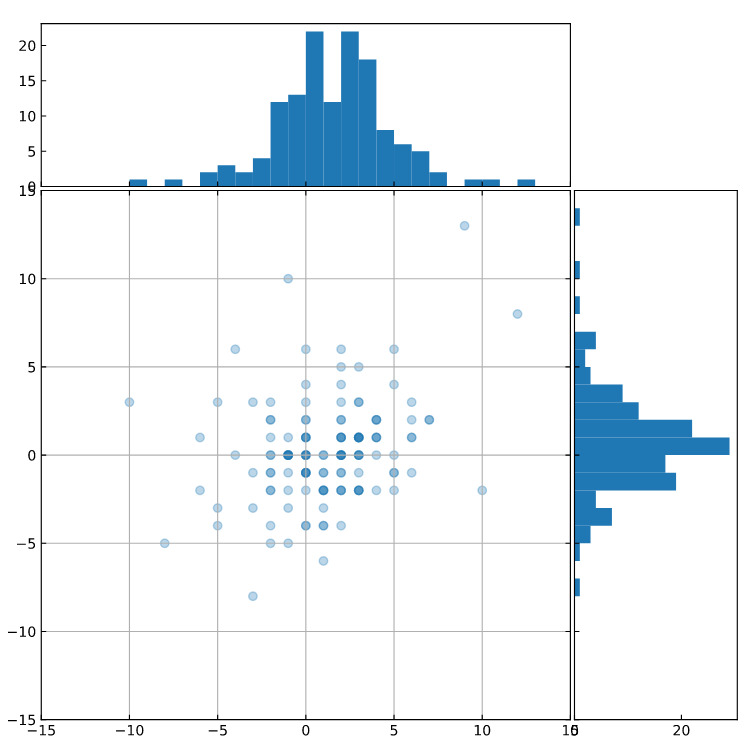
\includegraphics[width=.5\textwidth]{results_coord.jpeg}
	\caption{The x and y pixel deviations of all electrodes in the training dataset from the ground truth dataset.}
	\label{results_coord}
\end{figure}

\section{Discussion}
The use of a graph approach allows us to be less strict on the blob filtering tresholds. We considered a multitude of other cost functions (e.g. penalizing direction changes, infering likelihood of angles between specific electrode numbers using empirically determined anlge distributions, penalizing crossing edges) which we did't implement as satisfactory results were already achieved with only two features.


\section{Contributions}
\bibliography{references}
\bibliographystyle{apalike}
\end{document}